\documentclass[tikz, border=5pt]{standalone}

\begin{document}
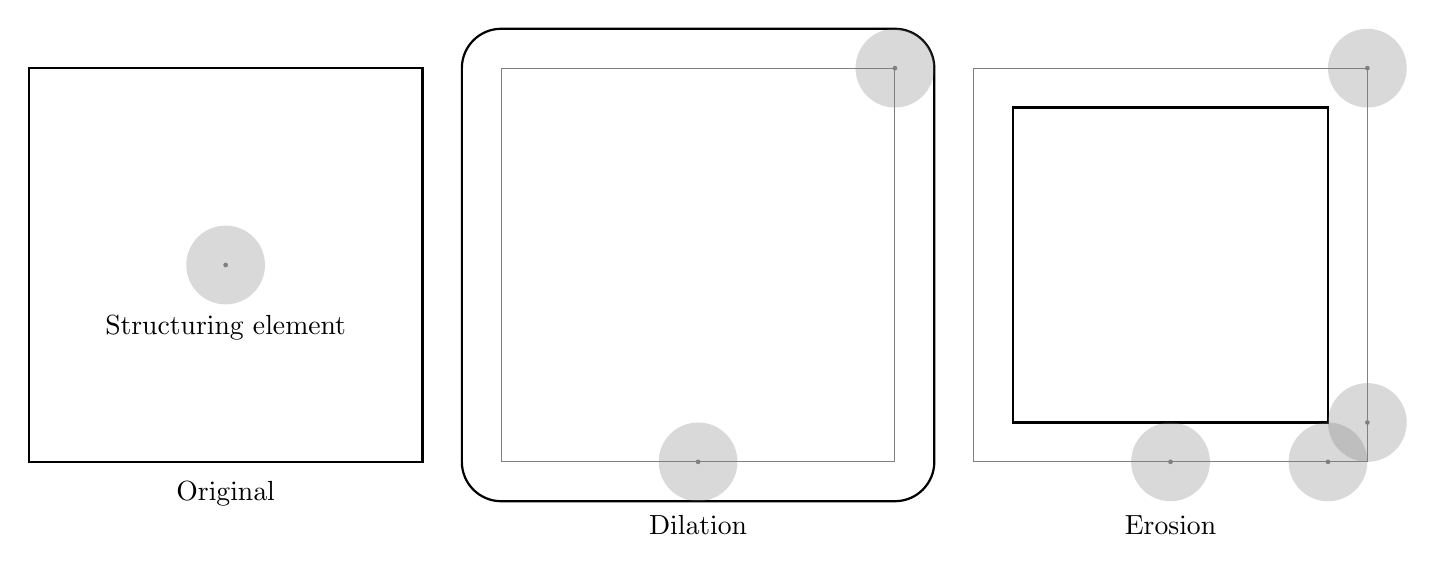
\begin{tikzpicture}

    %% Original
    \begin{scope}
        \draw[thick] (0, 0) rectangle (5,5);
        \node at (2.5, -0.4) {Original};
        \fill[gray, opacity=0.3] (2.5,2.5) circle(0.5);
        \node at (2.5, 1.7) {Structuring element};
        \fill[gray] (2.5,2.5) circle(0.03);
    \end{scope}

    %% Dilation
    \begin{scope}[xshift=6cm]
        \draw[gray] (0,0) rectangle (5,5);
        \node at (2.5, -0.8) {Dilation};
        \draw[thick, rounded corners=0.5cm] (-0.5,-0.5) rectangle (5.5,5.5);

        \fill[gray] (5,5) circle(0.03);
        \fill[gray, opacity=0.3] (5,5) circle(0.5);

        \fill[gray] (2.5,0) circle(0.03);
        \fill[gray, opacity=0.3] (2.5,0) circle(0.5);
    \end{scope}

    %% Erosion
    \begin{scope}[xshift=12cm]
        \draw[gray] (0, 0) rectangle (5,5);
        \node at (2.5, -0.8) {Erosion};
        \draw[thick] (0.5,0.5) rectangle (4.5,4.5);

        \fill[gray] (5,5) circle(0.03);
        \fill[gray, opacity=0.3] (5,5) circle(0.5);

        \fill[gray] (2.5,0) circle(0.03);
        \fill[gray, opacity=0.3] (2.5,0) circle(0.5);

        \fill[gray] (5,0.5) circle(0.03);
        \fill[gray, opacity=0.3] (5,0.5) circle(0.5);

        \fill[gray] (4.5,0) circle(0.03);
        \fill[gray, opacity=0.3] (4.5,0) circle(0.5);
    \end{scope}

\end{tikzpicture}
\end{document}
